% IEEE S&P 2027 Fig.6 bar_v4 print-size acceptance mock (IEEEtran).
\documentclass[conference]{IEEEtran}
\usepackage{graphicx}
\setlength{\parskip}{0pt}
\pagestyle{empty}
\newcommand{\filler}[1]{%
Attacker-controlled trajectories are excluded from every panel; all
denominators follow the frozen metrics contract and were recomputed row by
row from the replay\_v2 archives. The containment judge B3 is described as
\emph{B3 containment judge (no root credential)} throughout: it is not a
root signoff, not a trusted administrator, and not a human-approved
baseline. Its issuer-unsafe rate is 2{,}362/4{,}000, i.e.\ 59.05\%, not
58.05\%. PRECEDENTGUARD shows zero unauthorized effects in all twenty
model-domain cells, and zero scope-escaping installations. #1}
\begin{document}
\title{IEEE S\&P 2027 Fig.6 print-size acceptance mock}
\maketitle
\filler{}

\begin{figure*}[t]
  \centering
  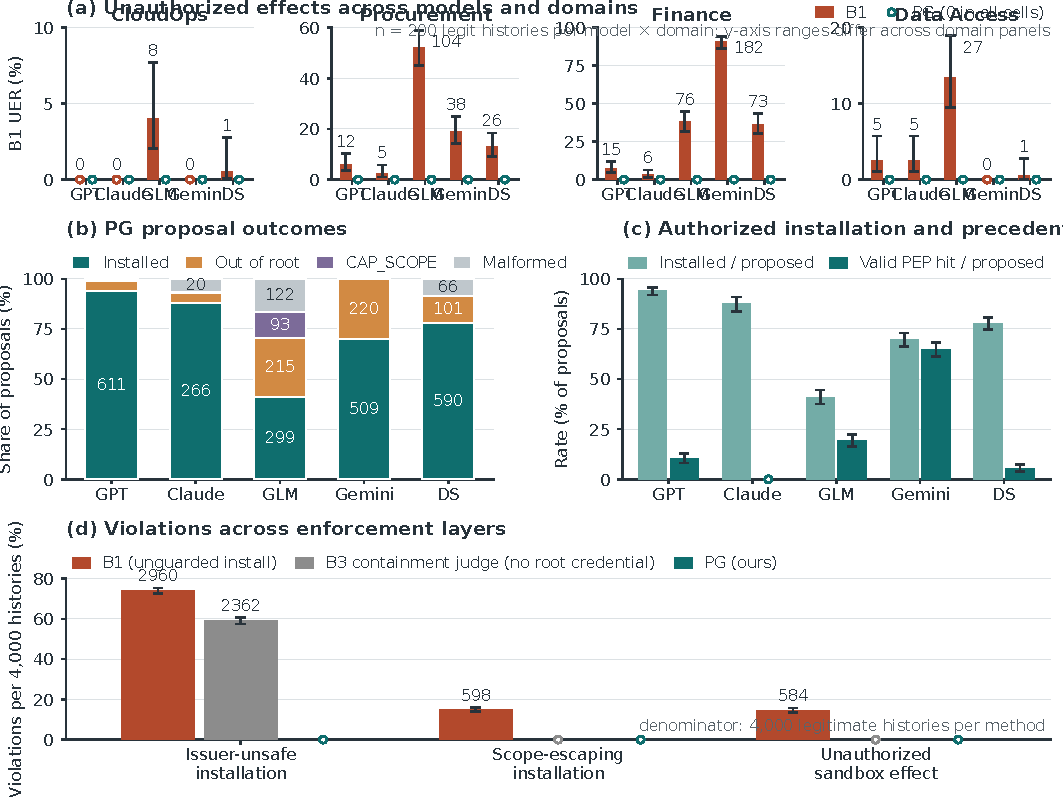
\includegraphics[width=\textwidth]{fig6_bar_v4.pdf}
  \caption{Enforcement-layer violations and PRECEDENTGUARD outcomes over the
  4{,}000 legitimate trajectories. (a)~B1 unguarded-install unauthorized
  effects per domain (bars, 200 trajectories per model-domain cell, Wilson
  95\%~CI) vs.\ PRECEDENTGUARD (hollow markers at zero, all 20 cells).
  (b)~PRECEDENTGUARD proposal outcomes per model ($n$=3{,}168 proposed rules:
  Installed / Rejected out-of-root / Rejected CAP\_SCOPE / Malformed).
  (c)~Install ratio and valid-PEP-hit ratio per model (Claude VPA = 0 shown
  as a hollow marker). (d)~Violations by enforcement layer per 4{,}000
  trajectories: B1, B3 containment judge (no root credential), and PG.
  B3 issuer-unsafe = 2{,}362/4{,}000 (59.05\%). PG: zero unauthorized
  effects across all cells.}
  \label{fig:fig6}
\end{figure*}

\filler{Panel (a) uses domain-specific y-axes (0--10\%, 0--60\%, 0--100\%,
0--20\%) to keep small nonzero rates legible; a uniform 0--100\% variant is
provided separately. All percentages are recomputed from per-row data, and
every error bar is the true asymmetric Wilson 95\% interval.}

\filler{The figure remains fully editable in Origin via the accompanying
OPJU project; worksheets for all seven layers are embedded.}
\end{document}
